
\subsection{Contours and Bounding Boxes}

Contours formally identify an object in a foreground mask by specifying the coordinates of its perimeter. This sub-process of the algorithm locates the contours for all foreground objects presented in the foreground mask it receives from the Morphology and Filtering sub-process. As output the this sub-process returns the bounding box coordinates of each foreground object. 

Figure \ref{fig:contour_polygon} shows the outlines of each foreground object from Figure \ref{fig:bounding_boxes} which were located by using OpenCV's findContours() function. The findContours function is based on the border following algorithm by Satoshi Suzuki \cite{satoshi_findContours} which seeks to locate the border of a connected component. Taking pixels at the extremities in the x and y direction for each contour is used to form bounding boxes as in Figure \ref{fig:bounding_boxes}. Bounding boxes can be used to determine the area, height, width and location of an object, which are important properties when trying to determine if an object is a vehicle, furthermore they store and compute more cheaply the irregular polygon of a contour. The bounding box dimensions and location are generated by the OpenCV function boundingRect() which takes a contour and returns the corresponding bounding box's up-right rectangle, that is the top left corner coordinate and the box's width and height. 


\begin{figure}[H]
    \centering
    \centering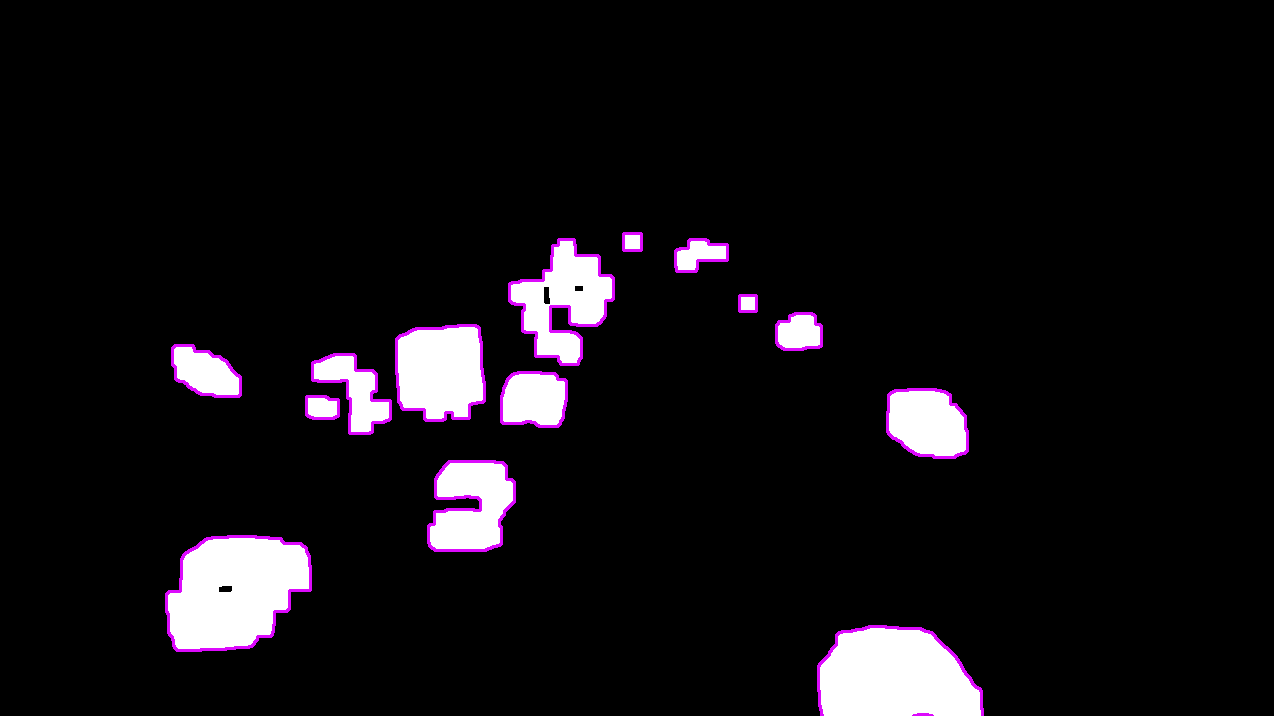
\includegraphics[width = 0.8\textwidth]{design/detection/bounding/mask_contours}
    \caption{Contours outlining foreground mask objects.}
    \label{fig:contour_polygon}
\end{figure}

\subsubsection{Calibration}

In order to reject foreground objects that are too large or small to be a vehicle bounding boxes should only be assigned to blobs which satisfy a specific size constraint. Blobs dimensions can be measured using the width and height of their contours. The limits on these dimensions should be set with the intention permitting the most vehicles and rejecting all other blobs. The calibration of the dimension limits depends on the camera perspective because a vehicle's perceived size changes as it moves toward and away from the camera. The region to focus on will be where the processes previous to this one (subtraction and morphology) have performed the best. Fortunately width and height are calculated for the extremities of a blob so its shape doesn't matter only its size which accommodates imperfect background subtraction.Figure \ref{fig:irreg_blob} shows foreground blobs that own a bounding box but are not at all shaped like a vehicle however their width and height satisfy the constraints. To select a specific height and width it's sufficient to simply measure the height and width of a variety of vehicle masks in the region of interest and then set the limits to accommodate those blobs. 


\begin{figure}[H]
    \centering
    \centering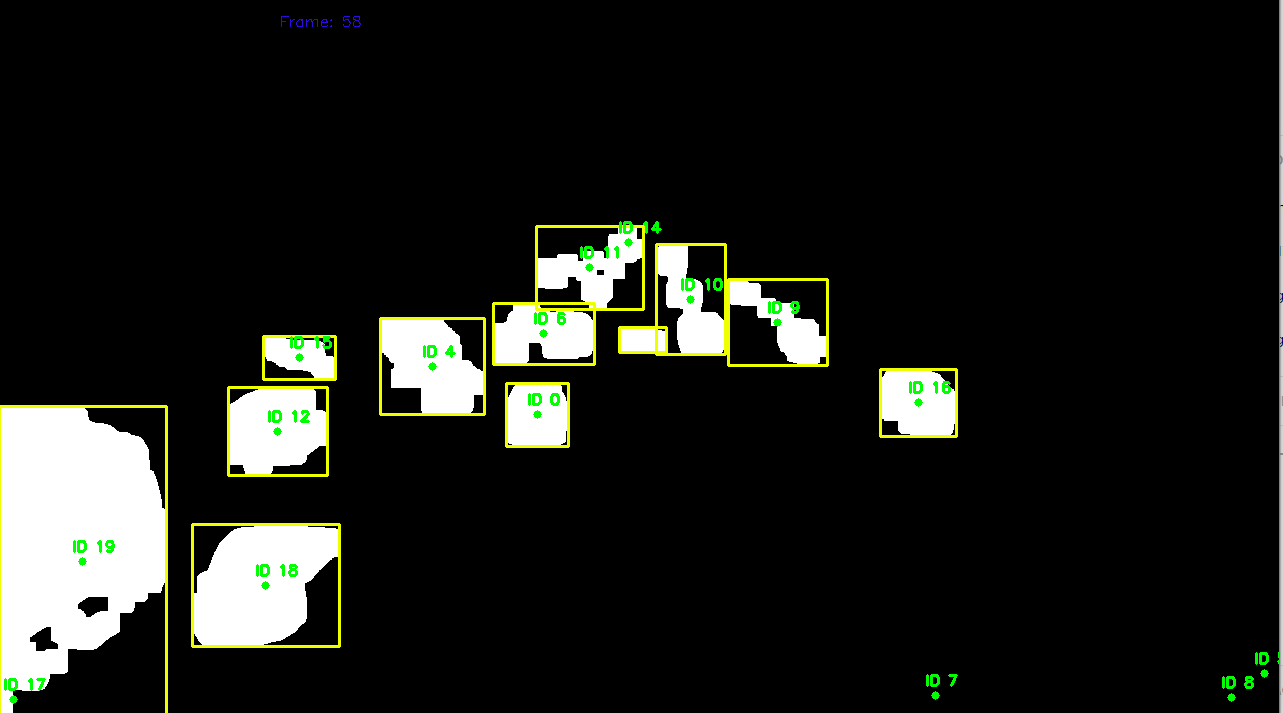
\includegraphics[width = 0.8\textwidth]{design/detection/calibration/irreg_blob_bound}
    \caption{Bounding boxes prescribed to irregular shaped blobs.}
    \label{fig:irreg_blob}
  \end{figure}

  

  
